
\documentclass[a4paper,11pt,twoside]{scrartcl}
\usepackage[utf8x]{inputenc}
\usepackage{graphicx}
\usepackage{geometry}
\usepackage[ngerman]{babel}
%\usepackage{babelbib}
%\usepackage[backend=biber]{biblatex}
\usepackage{units}
\usepackage{url}
\usepackage{setspace}
\usepackage[
	pdftitle={Energie_Suffizienz},
 	pdfauthor={et.al.},
% 	pdfsubject={},
% 	pdfkeywords={},
	pdfstartview=FitH, % Auf Seitenbreite anpassen (Anzeige)
	pdfborder={0 0 0},
%  	bookmarks=true,
% %	plainpages=false,
	colorlinks=false,
	hyperfootnotes=false,
	pagebackref=false]{}
\usepackage[colorinlistoftodos,prependcaption,textsize=normalsize]{todonotes}  % disable
\usepackage{amsmath}
\usepackage{amstext}
\usepackage{amssymb}
\usepackage{color}
\usepackage[numbers]{natbib}
\usepackage{pdfpages}
\usepackage{hyphenat}
\usepackage{pdflscape} % für drucken ändern auf package lscape /pdflscape
\usepackage{textpos}
\usepackage{microtype}
\usepackage{enumitem}
\usepackage{multirow}
\usepackage{pdfcomment}

\usepackage{pgfgantt} % gantchart für den Arbeitsplan

% \usepackage{hyphenat}
\usepackage{float}
\usepackage{placeins}
\RequirePackage[bf]{caption}

\renewcommand{\textfraction}{.01} % vorher: .2
\renewcommand{\floatpagefraction}{.99}% vorher: .5
\renewcommand{\topfraction}{0.9}	% max fraction of floats at top
\renewcommand{\bottomfraction}{0.9}	% max fraction of floats at bottom

\newcommand{\ltab}{\raggedleft\arraybackslash}
\newcommand{\ctab}{\centering\arraybackslash} 
\newcommand{\rtab}{\raggedright\arraybackslash}

\usepackage{tabularx}
\newcolumntype{L}[1]{>{\raggedright\arraybackslash}p{#1}} % linksbündig mit Breitenangabe
\newcolumntype{C}[1]{>{\centering\arraybackslash}p{#1}} % zentriert mit Breitenangabe
\newcolumntype{R}[1]{>{\raggedleft\arraybackslash}p{#1}} % rechtsbündig mit Breitenangabe

\newcommand{\rem}[1]{}

% \renewcommand{\figurename}{Abb.}
% \renewcommand{\tablename}{Tab.}

\usepackage{acronym}
%\renewcommand{\bflabel}[1]{\normalfont{\normalsize{#1}}\hfill}

\usepackage[automark]{scrpage2}
\pagestyle{scrheadings}
\clearscrheadfoot
\ohead{\headmark}
\ofoot{\pagemark}
\setheadsepline{0.4pt}
\setfootsepline{0.4pt}

\setkomafont{pageheadfoot}{\rmfamily\small}

\renewcommand{\thefigure}{\arabic{section}-\arabic{figure}}
\renewcommand{\thetable}{\arabic{section}-\arabic{table}}

\newcommand{\entspricht}{\mathrel{\widehat{=}}}

\geometry{left=25mm,right=25mm, top=25mm, bottom=28mm}
\parindent 0pt
\parskip 11pt

% kein Platz zwischen \items
\setlist{nosep}
% Platz nach Überschriften reduzieren
\usepackage{titlesec}
\titlespacing*{\section}{0pt}{0pt}{0pt}
\titlespacing*{\subsection}{0pt}{0pt}{0pt}
\titlespacing*{\subsubsection}{0pt}{0pt}{0pt}
\titlespacing*{\paragraph}{0pt}{0pt}{5pt} % horizontal spacing in paragraph

\begin{document}
\onehalfspacing

\clearpage


{\singlespacing

\thispagestyle{empty}
\begin{center}

%first row logos
\begin{figure}[htb]
    \centering
    \begin{minipage}[c]{0.3\linewidth}
        \centering
        
\includegraphics[width=4.5cm]{logos/europa-universitaet-flensburg-hauptlogo-rgb-600dpi.png}
    \end{minipage}
    \hfill
    \begin{minipage}[c]{0.35\linewidth}
        \centering
        \includegraphics[width=5cm]{logos/Logo_interdiszi_institut.png}
    \end{minipage}
    \hfill
    \begin{minipage}[c]{0.3\linewidth}
        \centering
        \includegraphics[width=2.5cm]{logos/Logo_wuppertal.png}
    \end{minipage}
\end{figure}

\iffalse
%second row logos
\begin{figure}[htb]
    \centering
    \begin{minipage}[c]{0.3\linewidth}
        \centering
        \includegraphics[width=2.2cm]{logos/2015_Logo_TUM_RGB.jpg}
    \end{minipage}
    \hfill
    \begin{minipage}[c]{0.35\linewidth}
        \centering
        \includegraphics[width=5.5cm]{logos/isea_rwth_logo.jpg}
    \end{minipage}
    \hfill
    \begin{minipage}[c]{0.3\linewidth}
        \centering
        \includegraphics[width=3cm]{logos/TU_Logo_lang_RGB_rot.png}
    \end{minipage}
\end{figure}
\fi
\vspace*{1 cm}

{\LARGE\textbf{\textsf{Skizze Nachwuchsforschungsgruppe}}

\textsf{\textit{im Rahmen der Bekanntmachung \glqq inter- und transdisziplinär arbeitende Nachwuchsgruppen im Rahmen der Sozial-ökologischen Forschung\grqq} }
}

\vspace{0.5cm}

{\Huge
\textbf{\textsf{Die Rolle von Energie-Suffizienz in Energiewende und Gesellschaft}}

\textbf{\textsf{}}
}

{\Huge
\textbf{\textsf{Akronym:{EnSufGe}}}
}

\vspace{1cm}

Eingereicht durch
Frauke Wiese\\
i$^{2}$ Interdisziplinäres Institut für Umwelt-, Human- und Sozialwissenschaften\\
Europa-Universität Flensburg, Auf dem Campus 1, 24943 Flensburg


\vspace{0.5cm}

An den Projektträger im DLR \\
AE 41 Globaler Wandel/Klima- und Umweltschutz, Sozial-ökologische Forschung \\
Heinrich-Konen-Straße 1, 53227 Bonn


\end{center}
\iffalse
\begin{table*}[b]
\centering
\footnotesize
\begin{tabular}{ | p{5cm} | p{5cm} |} \hline
\textbf{Konsortialpartner} & \textbf{Modelle/Frameworks} \\ \hline
Reiner Lemoine Institut & Leitung des Experiments \\ \hline
Technische Universität München & urbs \\ \hline
Europa-Universität Flensburg & oemof \\ \hline
RWTH Aachen & GENESYS-2 \\ \hline
Technische Universität Berlin & OSeMOSYS \\ \hline
Dänische Technische Universität & Balmorel \\ \hline
\end{tabular}
\label{tab:Partner}
\end{table*}
\fi


\clearpage
}

\setcounter{page}{1}

\section*{Kurzfassung für easy-Formular}
%Bitte beschreiben Sie Ihr Vorhaben kurz und prägnant. Die Gliederung soll das Vorhabenziel, die geplante Vorgehensweise bzw. Arbeitsplanung sowie den möglichen gesellschaftlichen Nutzen der Ergebnisse enthalten. Es stehen Ihnen insgesamt maximal 2000 Zeichen zur Verfügung (Leerzeichen, Zeilenumbrüche und ähnliche eingerechnet).

\section{Zielstellung und gesellschaftlicher Bedarf}
\label{sec:ziel}
%\textit{Beschreibung der Problem- und Zielstellung sowie des gesellschaftlichen Bedarfs}

In Anlehnung an Albert Einstein liegt der Ausgangspunkt des Nachwuchsforschungsvorhabens darin, dass Probleme nicht mit derselben Rationalität gelöst werden können, die sie hervorgebracht haben. Zwar ist die zentrale Herausforderung einer Energiewende in Deutschland angesichts von Klimawandel, Ressourcenverknappung und Risikotechnologien erkannt, doch die Debatten und Maßnahmen verbleiben überwiegend in alten Rationalitätsmustern: Die Energiewende wird unter den Aspekten von Kosten, Marktpotenzialen (einschließlich neuen Geschäftsfeldern) und technischer Machbarkeit (Effizienz und Konsistenz) debattiert, während „Treiber“ vermehrten Energieverbrauchs, wie das Wachstumsparadigma oder zunehmende Innovationsgeschwindigkeit, kaum problematisiert werden. Energiesystem-Modelle haben sich als Werkzeuge etabliert, um technisch mögliche und ökonomisch vorteilhafte Energiewende-Pfade im Zusammenspiel von Effizienz- und Konsistenz-Strategien abzubilden. Entwicklungen, die eine Reduktion des absoluten Energieverbrauchs durch veränderte Praktiken und Routinen im Sinne einer Suffizienz-Strategie ermöglichen, werden bisher kaum berücksichtigt \cite{SAMADI2017}. Die Nachfrage-Seite wird in bestehenden Modellen meist höchstens über technologische Änderungen (Effizienzmaßnahmen) abgebildet, die Nachfrage selbst in der Regel jedoch nicht hinterfragt \cite{Creutzig2018}, meist nur innerhalb enger Grenzen variiert und die dahinter liegenden Annahmen auch dann nicht explizit gemacht. Ein entscheidender Einflussparameter für berechnete Szenarien ist aber die zukünftige Nachfrage nach Strom, Wärme und Mobilität. Mit anderen Worten: Bislang sind Modellierungen weitgehend blind gegenüber Veränderungen durch gesellschaftlichen Wandel oder im Verhalten und berücksichtigen hier liegende Potenziale und Risiken nicht. Zudem bleiben eng mit der Energiewende verknüpfte Aspekte wie Flächenverbrauch, Ressourcenbedarf \cite{Mocker2015,Buchert2011} und Akzeptanzfragen \cite{Fuchs2016}, zusammengefasst die Einhaltung der planetaren Grenzen \cite{Rockstroem2009} und eine nachhaltige Entwicklung im Sinne der Sustainable Development Goals \cite{UN_SDG} unberücksichtigt.\\
Vor diesem Hintergrund liegt das übergreifende Ziel des angestrebten Nachwuchsverbundes darin, Suffizienzaspekte und -strategien für die Energiesystem-Modellierung zu operationalisieren und damit verhaltensbasierte Parameter und gesellschaftlichen Wandel in Energie- und Klimaschutzszenarien abbildbar zu machen. Die Parameter werden dabei mit Instrumenten, Handlungsoptionen und veränderten Rahmenbedingungen explizit hinterlegt. Hierfür gilt es, gesellschaftliche Transformationsprozesse im Kontext der Energiewende besser zu verstehen, die Blockaden für und Potenziale von Suffizienzpolitiken auszuloten und nicht zuletzt im Sinne einer globalen Nachhaltigkeit mögliche Externalisierung und Verlagerungseffekte zu diskutieren.

\begin{table}[h]
\begin{center}
\small
  \caption{Bedeutung der Begriffe in Bezug auf Energiewende}
\begin{tabular}[h]{|l | l |}
\hline
&\\
Konsistenz & Erneuerbare Energien ersetzen Fossile\\
&\\
\hline
&\\
 Effizienz & relative Reduktion des Energieverbrauchs bei Bereitstellung der gleichen\\
 & Energiedienstleistung\\
 \hline
 &\\
Suffizienz & absolute Reduktion des Energieverbrauchs durch soziale Innovationen, Exnovationen\\
& und verändertes Nutzungsverhalten \\
 \hline
 \end{tabular}
 \label{tab:koefsu}
\end{center}
\end{table}

\section{Stand von Wissenschaft und Technik sowie eigene Vorarbeiten}
\label{sec:2}

% gemeinsamer Anfang 
Nachhaltigkeitsforschung, sozial-ökologische Forschung und Transformationsforschung sind seit langem mit Fragen der Umsetzung befasst: Wie ist es möglich, vom Wissen zum Handeln zu kommen ? \cite{BMBF2008} Wie kann geschehen, was geschehen muss ? \cite{Linz2000} Und wie können Klimaschutzziele, wie kann ein deutlich geringerer Naturverbrauch erreicht werden, ohne zivilisatorische Errungenschaften zu gefährden ? \cite{Sommer2016,WGBU2011} Die Antworten fallen unterschiedlich aus und die Bearbeitung dieser Frage geschieht in unterschiedlicher Weise.

\subsection*{Energiesystem-Analyse und Modellierung}
% ROlle Modelle
Energiesystem-Modelle sind Werkzeuge um  Orientierungswissen zu Energiewendepfaden zu generieren. So wurden mit ihrer Hilfe die Realisierbarkeit von 100\% Erneuerbare Energien Strom-Systemen dargelegt, sowohl für Deutschland \cite{SRU2011} als auch für Europa \cite{Hohmeyer2015}. Inzwischen geht es in der ökonomisch-technisch geprägten Energiesystem-Analyse nicht mehr um das OB, sondern eher um das WIE der Energiewende und  eine steigende Anzahl komplexer Modelle wird genutzt, um Chancen der Sektorkopplung von Strom, Wärme, Mobilität \cite{Quaschning2016} einzuschätzen, Marktregeln bei hohem Anteil Erneuerbarer Energien zu erörtern, sowie Netz- \cite{openEgo2015} und Speicherbedarf \cite{ANGUS2017} abzuschätzen.
% ESM wichtig in Politik-Beratung
Zu Richtungsentscheidungen für Energiewendepfade nehmen Energiesystem-Modelle somit eine wichtige Rolle in Wissenschaft und politischer Beratung zu Klima- und Energiepolitik ein. \cite{Dieckhoff2015}.\\
% Transparenz wichtig für Partizipation wichtig
In den letzten Jahren werden die Modelle jedoch verstärkt für ihren Black-Box-Charakter kritisiert \cite{Pfenninger2017, Pfenninger2017b,Cao2016}. \citep{Wiese2015} formuliert den Bedarf an Transparenz in der Energiesystem-Modellierung um Partizipation zu ermöglichen \cite{Wiese2014} als Grundlage für Transparenz, die essentiell für eine partizipative Energiewende ist.
% Interdisziplinär wichtig, Sozialwissenschaft unterrepräsentiert
Außerdem wird zunehmend ein Bedarf an interdisziplinären Ansätzen in der Energiesystem-Modellierung identifiziert \cite{Wiese2018,Pfenninger2014,Schuitema2017}. Die  Sozialwissenschaften sind für eine gesellschaftliche Energiewende von großer Bedeutung \cite{Sovacool2015}, jedoch völlig unterrepräsentiert in der Energieforschung \cite{Sovacool2014}.\\
% Sozialwissenschaftliche Ansätze bisher (stärker Arbeiten EUM/Frauke herausarbeiten)
Die Energiesystem-Analyse an der EUF trägt mit der Bereitstellung von offenen Modellen \cite{renpass,renpassGIS} und einem Modellierungs-Framework \cite{oemof} zu der nötigen Transparenz der Energiesystem-Analyse bei. Im Projekt "vernetzen" \cite{vernetzen2016} wurde die Verknüpfung von sozialwissenschatlichen Ansätzen mit der Energiewende-Modellierung in Bezug auf Akzeptanz von Windkraftanlagen und Netzausbau erprobt. Die Energiemodellierung als Werkzeug wird im Hinblick auf ihre Nützlichkeit von den Modellierer*innen selbst beständig hinterfragt \cite{Wiese2018}.  %Außerdem beschäftigte \citep{Wiese2016} sich mit der Perspektive der Resilienz als verknüpfendes Element in der ESA.  und legt bei der Erstellung von Klimaschutzprojekten den Fokus auf die Beteilung der lokalen Akteure (REFERENZ).

\subsection*{Sozial-ökologische Transformationsforschung}

% Energiewende geht, aber geschieht nicht - gesellschaftliche Gründe
Dass die Etablierung einer klimafreundlichen und nachhaltigen Energieversorgung grundsätzlich technisch machbar und ökonomisch zu bewältigen wäre, stellt die Energiesystem-Modellierung immer wieder dar. Dafür, dass dies nicht in der gebotenen Geschwindigkeit geschieht, werden vor allem gesellschaftliche Barrieren und Zwänge ausgemacht.
% hier hilft die SÖTF
In der sozial-ökologischen Transformationsforschung werden gesellschaftliche Transformationsprozesse -- wie die Transformation des Energieregimes -- als zukunftsorientierte Gestaltungsaufgabe verstanden \cite{Sommer2016}. In der Energiewende spielt Suffizienz bislang noch eine untergeordnete Rolle – obwohl die Reflektion der bis dato ergriffenen Maßnahmen zeigt, dass diese zur Senkung des absoluten Verbrauchs nicht ausreichen werden \cite{Brischke2016}. Ohne Suffizienz wird die Energiewende, das wird in der sozial-ökologischen Forschung seit längerer Zeit thematisiert, nicht zu schaffen sein \cite{Huber1995,Fischer2013,Schneidewind2013}.\\
% Beitrag NEC
Am Norbert Elias Center for Transformation Design & Research (NEC) werden historische Prozesse umfassenden gesellschaftlichen Wandels rekonstruiert, um aus den gewonnenen Erkenntnissen Handlungsoptionen, mögliche Entwicklungslinien und Gestaltungsszenarien für zeitgenössische und künftige sozial-ökologische Wandlungsprozesse abzuleiten \cite{Christ2015,Christ2016}, als auch gegenwartsorientierte Fragestellungen zum Zusammenhang von Klima, Kultur und Nachhaltigkeit bearbeitet \cite{Sommer2011,Sommer2015,Stumpf2015}.\\
% NEC Suffizienz-Projekt - Projekte zusammenfassen
Als Strategie die auf veränderte Handlungsmuster und Nutzungsaspekte zielt, steht Suffizienz im Fokus des BMBF geförderten Forschungsprojekts „Entwicklungschancen und -hemmnisse einer suffizienzorientierten Stadtentwicklung (EHSS)“ (2017-2020).
% In diesem Forschungsprojekt werden in vergleichender Perspektive und im Rahmen eines Reallabors auf kommunaler Ebene Erfolgsbedingungen und Barrieren suffizienzorientierter Stadtentwicklung untersucht. Eine Suffizienzpolitik in der Stadtentwicklung schafft Strukturen, die suffizienzorientierte (Alltags-) Praktiken erleichtern – etwa im Bereich der Mobilität, des Wohnens oder der Ernährung.
% NEC Gemeinwohlprojekt
Auch im Rahmen des BMBF-geförderten Forschungsprojekts „Gemeinwohl-Ökonomie im Vergleich unternehmerischer Nachhaltigkeitsstrategien (GIVUN)“ (2015-2018) wurden Fragen der Suffizienz thematisiert, etwa bezüglich der Frage, wie stark diese bzw. eine absolute Reduktion des Ressourcenverbrauchs von verschiedenen Instrumenten unternehmerischer Verantwortung adressiert und eingefordert wird \cite{Sommer2016b}.
% NEC Gute Beispiele nachhaltigen Handelns, auch Suffizienz im Projekt
Auch das vom Umweltbundesamt geförderte Forschungsprojekt "Von der Nische in den Mainstream. Wie gute Beispiele nachhaltigen Handelns in einem breiten gesellschaftlichen Kontext verankert werden können." beschäftigte sich u.a. mit Suffizienzorientierungen und -strategien \cite{Kny2015}.
    
\subsection*{Sufizienzpolitik}

% Politische Dimension Suffizienz
Als Nachhaltigkeits-Strategie mit einer politischen Dimension ist Suffizienz lange kaum debattiert worden \cite{Winterfeld2002}. Erst im Kontext der ab 2010 sich neu entzündenden wachstumskritischen Debatte wurde der Begriff vermehrt aufgegriffen und bearbeitet (REFERENZEN siehe u.a. Seidl/ Zahrnt 2010 REFERENZ; Rätz/ von Egan-Krieger 2011; und Adler/ Schachtschneider 2017), \cite{Schneidewind2013,Winterfeld2017,Linz2015,Bierwirth2015,Thomas2015}. Die internationale Debatte zu Suffizienzpolitiken wird stark durch den ökofeministischen Ansatz von REFERENZ Ariel Salleh (2009) mit geprägt und ergänzt aus der Perspektive des globalen Südens den Ansatz des „Savings“ (das Recht, etwas übrig zu behalten im Kontext der Armutsbekämpfung).\\
% WI: Suffizienz verankert - LISTE IM ANHANG?
Die Suffizienz-Forschung und Arbeit zu Suffizienzpolitik ist am WI seit vielen Jahren verankert (vgl. Verweise auf Wolfgang Sachs, Manfred Linz, Uwe Schneidewind u.a.).
% WI Projekte SUffizienz
Neben den genannten Publikationen umfassten die Arbeiten zu diesem Thema in den letzten Jahren insbesondere das Projekt „Energiesuffizienz“ \cite{Brischke2016} im Rahmen der Sozial-ökologischen Forschung des BMBF sowie das Projekt „Policy Guide: Energy Sufficiency in Buildings“ \cite{EnergySufficiencyProjekt} zur Entwicklung suffizienzpolitischer Maßnahmen für die europäische Ebene.
% WI Projekte inter und trans, methodisch integr. sozial in Modell
Darüber hinaus bestehen umfangreiche Erfahrungen in der Bearbeitung inter- und transdisziplinärer Projekte, wie etwas das Partizipationskonzept des Klimaschutzplans NRW \cite{Klimaschutzplan2011,Klimaschutzplan2012}, der interdisziplinären Modellierung im Rahmen des Projektes COMBI \cite{COMBI2015} sowie in der methodischen Entwicklung zur Integration sozialwissenschaftlicher Empirie in die Modellierung \cite{Bierwirth2016}.||
% Suffizienz in Modellen bisher kaum, schwierig, nötig
Während die Integration von Suffizienzpolitiken und Transformationserzählungen in Ansätzen schon erfolgt, stellt die suffizienzbasierte Modellierung eine noch kaum abschätzbare Herausforderung dar \cite{SAMADI2017}. Eine gelungene inter- und transdisziplinäre Verkopplung aller drei Teilbereiche bedarf neben neuer Theorieansätze (z.B. zur „Externalisierung“) auch neuer methodologischer und methodischer Ansätze einschließlich quantitativ-qualitativer Verkopplungen.

\section{Bezug zur Sozial-ökologischen Forschung und zu den Förderzielen}

% Bezug zu Sozial-ökologischer Forschung
% inderdisziplinär
Erster Bezugspunkt zur sozial-ökologischen Forschung ist die Interdisziplinarität des beabsichtigten Nachwuchsforschungsverbundes. Sie soll insbesondere über die Zusammenarbeit von Technik- und Sozialwissenschaftler*innen erfolgen (zur disziplinären Zusammensetzung siehe Abschnitt \ref{sec:4}). Mit der Weiterenwicklung interdisziplinärer Szenario-Methoden und deren Anwendung trägt die Nachwuchsforschungsgruppe zur Integration disziplinären Wissens für Energiewende und Klimaschutz bei.\\
% transdisziplinär
Zweiter Bezugspunkt ist der transdisziplinäre Ansatz, eng mit Praxispartner*innen zu kooperieren und hier auf den qualitativen und innovativen methodischen Ansatz der „transdisziplinären Erzählungen“ (REFERENZ Biesecker, Breitenbach Winterfeld 2016) zurückgreifen zu können. Diese sind auch für die lebensweltliche Einbettung des Vorhabens besonders geeignet. Im Projekt ist eine enge Zusammenarbeit mit kommunalen Praxispartnern bei der Szenarienerstellung und -bewertung vorgesehen, wobei auf bestehende Kooperationen aufgebaut werden kann (siehe Abschnitt \ref{sec:5}).\\
% international und gender
Weiter und in Bezug zu den Förderzielen soll sowohl die internationale Dimension (z.B. Auswirkungen deutscher Energiewendepolitiken auf andere Länder) als auch der über die Integration der Genderdimension mögliche Perspektivwechsel in den Promotionsvorhaben bearbeitet werden.\\
% Inhaltlicher Bezugspunkt zu SOEF
Theamtisch widmet sich die Nachwuchsforschungsgruppe einer in der Sozial-ökologischen Forschung als zentral geltenden Nachhaltigkeits-Herausforderung: Der umwelt- und gesellschaftsverträglichen Transformation des Energiesystems. Mit der Fokussierung auf Suffzienz nehmen die Nachwuchswissenschaftler*innen Bezug zu Ressourcenschonung sowie dem Sozial-ökologischen Forschungs-Schwerpunkt Nachhaltiges Wirtschaften.\\
% Bezug zu Förderzielen: Institutionell und Kooperation außeruniversitär
Die Weiterentwicklung institutioneller Kapazitäten zur Durchführung transdisziplinärer Nachhaltigkeitsforschung wird durch die Verankerung der Nachwuchsgruppe am Interdisziplinären Institut für Umwelt-, Sozial und Humanwissenschaften an der Europa-Universität Flensburg (EUF) sowie am Wuppertal Institut (WI) geschaffen. Der Wissensaustausch zwischen Hochschule und außeruniversitärer Forschungseinrichtung wird verstärkt durch die gemeinsame Leitung von Wissenschaftler*innen beider Institutionen (siehe Abschnitt \ref{sec:5}). In der eigenverantwortlichen Arbeitsgruppe bekommen junge Wissenschaftler*innen die Möglichkeit sich auf der Basis ihres disziplinären Vorwissens Sozial-ökologischen Fragestellungen zu widmen. Möglichkeiten zur Weiterqualifizierung werden durch die Nachwuchsgruppe für wissenschaftliche Mitarbeiter*innen geschaffen, die zwar schon jetzt an den Schnittstellen forschen, dafür aber nicht den entsprechenden Rahmen haben um sich auch wissenschaftlich zu qualifizieren.

\section{Forschungsarbeit und Arbeitsprogramm}
\label{sec:4}
%\textit{Beschreibung der geplanten Forschungsarbeiten und des Arbeitsprogramms, unter Einschluss der Darstellung von Methoden, die zur Anwendung kommen bzw. entwickelt werden sollen; sowie der disziplinären Zusammensetzung der geplanten Nachwuchsgruppe}\\
%\textit{FRAGE: Methoden, Disziplinen als Unterpunkte?}\\

\begin{figure}[!h]
    \centering
    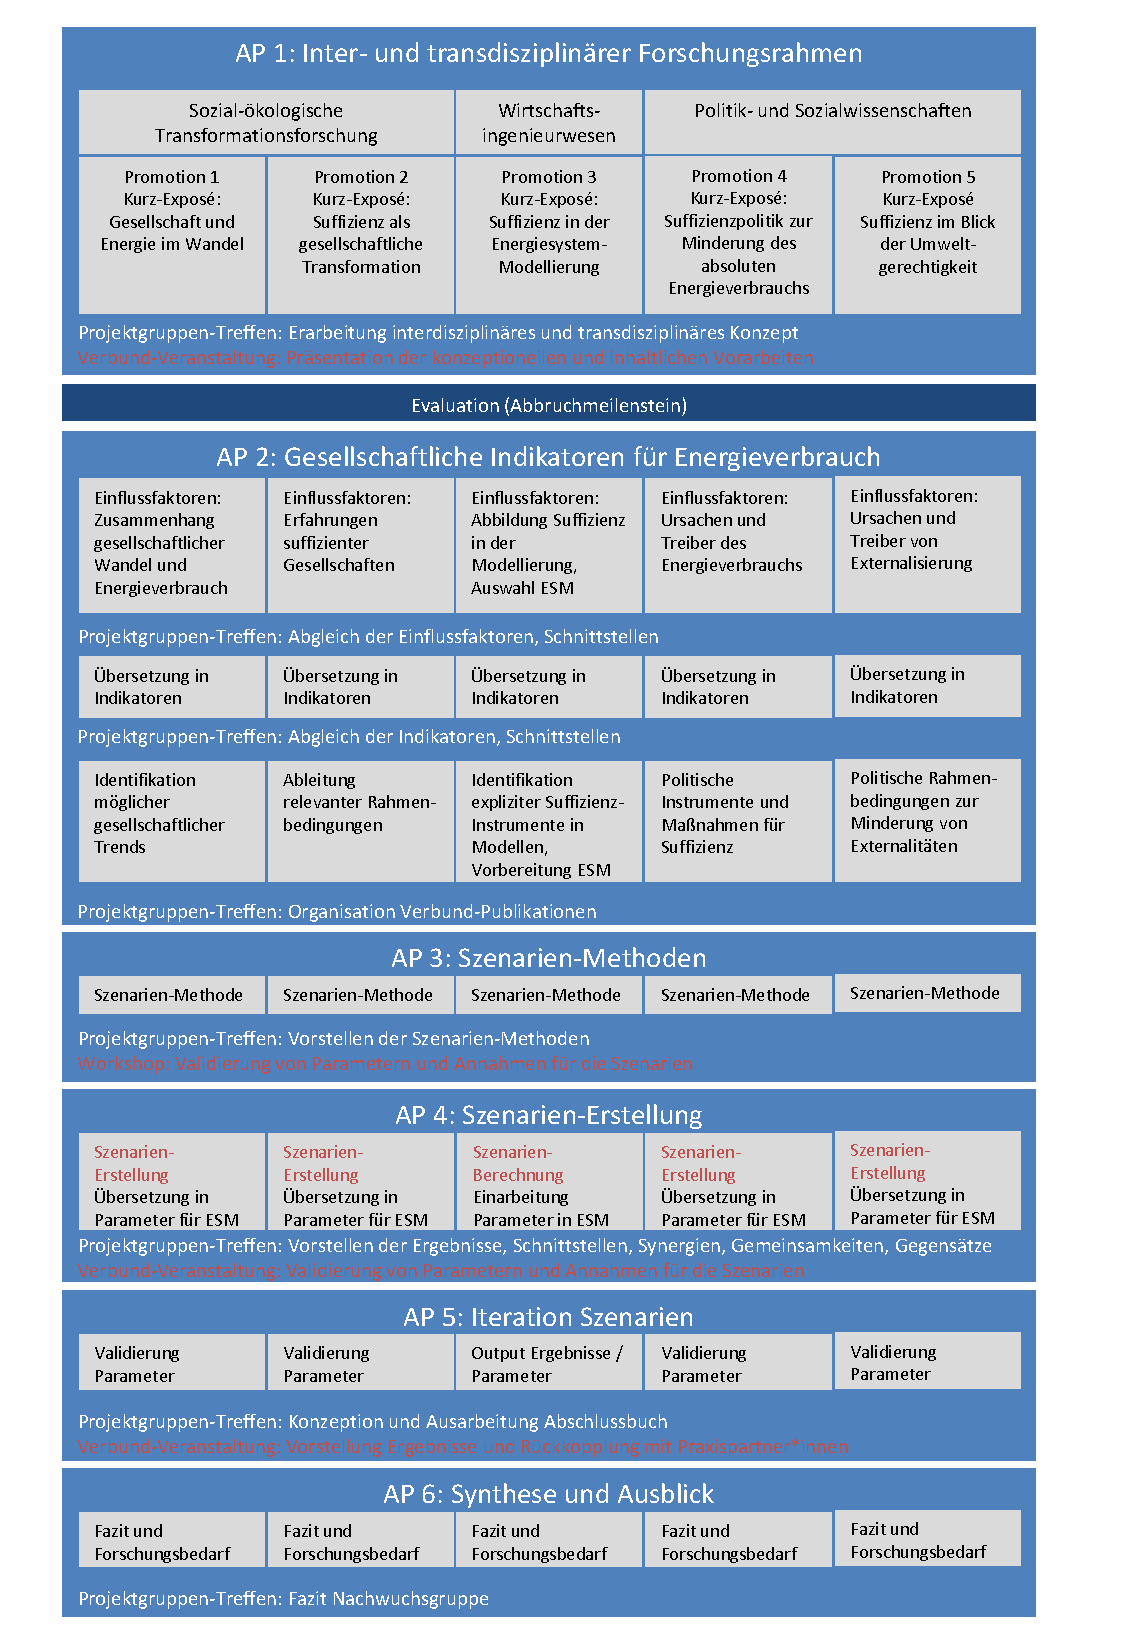
\includegraphics[width=0.9\textwidth]{figures/Forschungsarbeit3.pdf}
    \caption{Forschungsprogramm der Nachwuchsforschungsgruppe}
    \label{fig:forschungsprogramm}
\end{figure}

Abbildung \ref{fig:forschungsprogramm} skizziert die fünf Promotionsvorhaben (vertikal dargestellt) in drei Forschungs-Schwerpunkten, die über die sechs interdisziplinären Arbeitspakete (horizontal dargestellt) ineinander greifen.

\subsection{Forschungs-Schwerpunkte und Disziplinen}
%sozial-ökologische Transformationsforschung: Gesellschaftlicher Wandel und Energieverbrauch}
%Vergangene umfassende gesellschaftliche Transformationen sind immer mit einer Veränderung der energetischen Basis von Gesellschaften einher gegangen, dies ist in der sozial-ökologischen Forschung verschiedentlich herausgearbeitet worden. 
Es sind zwei Promotionen sind im Bereich der sozial-ökologischen Transformationsforschung vorgesehen. Während die eine am NEC angesiedelte Promotion in historischer Perspektive Zusammenhänge zwischen Energieverbrauch und sozialem Wandel herausarbeiten wird, ist die zweite Arbeit dem Blick in wahrscheinliche, mögliche und wünschbare Zukünfte (REFERENZ Kreibich 2008) und der Frage gewidmet, wie gesellschaftliche Veränderungen und Trends künftig mit Energieverfügbarkeit und -nachfrage interagieren werden. Aus beiden zeitlichen Perspektiven – der historischen Rekonstruktion wie dem Blick auf wahrscheinliche, mögliche und wünschbare Zukünfte – werden sich Möglichkeiten und Grenzen (etwa aufgrund von Pfadab-hängigkeiten, nichtintendierten Nebenfolgen, Rebound etc.) für einen suffizienten Umgang mit Energie bzw. eine absolute Reduktion des Energieverbrauchs ableiten lassen.

%Ausgehend von bestehenden Szenarien und Erzählungen aus der sozial-ökologischen Forschung (WBCSD 1997; WBGU 2011; Öko-Institut 2017) bzw. der Sozialforschung (Wallerstein et al. 2014) werden unter anderem folgende Fragen gestellt: Mit welchen Auswirkungen gesellschaftlicher Entwicklungen etwa im Bereich der Demographie, der Migration oder der Digitalisierung auf Wohnflächennutzung (und damit Wärmebedarf), Mobilität oder Strom etc. ist zu rechnen? Welche Zukünfte bzw. Zukunftsszenarien sind sonst noch möglich? Was sind jeweils zu erwartende Implikationen für Energieverbräuche und welche Potenziale der Energie-Suffizienz beinhalten sie?

%\subsection*{Forschungs-Schwerpunkt Suffizienz-Politik und Energiewende}
Der Forschungs-Schwerpunkt Suffizienz-Politik und Energiewende ist am WI verortet und wird von Benjamin Best geleitet. Hierin sollen zwei Promotionen mit sozial- bzw. politikwissenschaftlichem Hintergrund entstehen.\\ 
Eine Dissertation beschäftigt sich mit der Gestaltung von politischen Rahmenbedingungen und ihren Wechselwirkungen auf energierelevanten sozialen Praktiken, Verhaltensweisen und Routinen. Die übergeordnete Fragestellung wird sein, inwiefern Politik und veränderte Rahmenbedingungen suffizientes Verhalten befördern, behindern oder allgemein beeinflussen können.\\
Das zweite Promotionsvorhaben in diesem Bereich ist im noch jungen und in Deutschland vergleichsweise wenig verbreiteten Ansatz der Politischen Ökologie angesiedelt. Ausgangspunkte sind „Imperiale Lebensweisen“ \cite{Brand2017}und Externalisierung (REFERENZ Lessenich; Biesecker; Winterfeld). Es soll untersuchen, inwiefern Suffizienzpolitiken zur Veränderung dieser Grundkonstellationen beitragen können und stellt damit die übergeordnete Forschungsfrage der Nachwuchsgruppe in einen internationalen Kontext (vgl. 2.1 der Förderbekanntmachung).

%\subsection*{Forschungs-Schwerpunkt Energiesystem-Analyse: Suffizienz in der Energiesystem-Modellierung}
Unter der Leitung von Frauke Wiese wird sich ein*e Doktorand*in mit wirtschaftsingenieurs-wissenschaftlichem Hintergrund auf die Abbildung von Suffizienz in Energiesystem-Modellen fokussieren. Das Promotionsvorhaben umfasst sowohl die Methodik Indiktoren aus dem sozialwissenschaftlichen Bereich in einem quantitativen Modell abzubilden als auch die Berechnung von Energie-Szenarien, die Suffizienz neben Effizienz- und Konsistenz-Optionen abbilden. Die Modellierung soll auf auf einem bestehenden offenen Modell aufbauen und dieses um den Aspekt Suffizienz erweitern. Ob hierfür das u.a an der EUF erarbeitete Energiesystem-Modellierungs-Framework 'oemof' in der Nachwuchsgruppe genutzt und erweitert wird, bleibt einer genauen Prüfung und dem Vergleich mit anderen Optionen vorenthalten.

\subsection{Arbeitspakete und Methoden}
\subsubsection*{AP1: Inter- und transdisziplinärer Forschungsrahmen}
% allgemein Bezugsrahmen
Zu Beginn der fünf Jahre wird von allen Gruppenmitgliedern der interdisziplinäre Bezugsrahmen für Forschung zu Energie-Suffizienz %aus Sicht der Energiesystemanalyse, der sozial-ökologischen Transformationsforschung und der Sozial- und Politikwissenschaften
entworfen. Im Rahmen eines Auftakt-Workshops mit den Promovenden werden die bis dahin zu erstellenden Skizzen zu Promotionsideen vorgestellt und diskutiert.
% fokussierung promotionen und wie trotzdem gemeinsam
In diesem Zusammenhang wird ausgelotet, inwiefern eine inhaltliche, thematische oder sektorale Fokussierung in einzelnen Promotionen sinnvoll oder notwendig ist (z.B. Privathaushalte, Mobilität, spezifische Zielgruppen, geografische Verortung). Diese gemeinsame inhaltliche Abstimmung ist grundlegend für die weitere Bearbeitung, um eine interdisziplinäre Arbeitsweise der Gruppe auch bei evtl. Schwerpunktsetzung sicherzustellen und ausschließlich multidisziplinäre Ergebnisse zu vermeiden.
% auch organisatorisch
Neben der inhaltlichen Abstimmung wird in diesem Rahmen die Zusammenarbeit auch organisatorisch geplant.\\
%Im Ergebnis wird ein Konzept erarbeitet, das die Synthesephasen, die Organisation und Ergebnisse der interdisziplinären Arbeit (z.B. gemeinsame Publikationen und Vorträge auf nationalen und internationalen Konferenzen ) darstellt.\\
Ein weiteres Ziel von AP 1 ist die gemeinsame Entwicklung eines transdisziplinären Forschungsdesigns. 
%Dies bezieht sich sowohl auf die einzelnen Promotionen wie auch auf die interdisziplinären Synthesephasen.
Die Promovenden definieren, welche Akteure sie wie im Rahmen ihrer Doktorarbeit beteiligen. %Die Beteiligungskonzepte werden vor dem Hintergrund der jeweiligen Fragestellungen und Zielgruppen in den skizzierten Arbeiten voraussichtlich unterschiedlich ausfallen. 
Im Rahmen eines zweiten gemeinsamen Workshops werden darauf aufbauend Ideen generiert, wer in welcher Form im Rahmen eines Beteiligungsprozesses über die Gesamtlaufzeit einzubinden ist.
%, wie dieser organisiert werden kann und welche Formate der Beteiligung sich anbieten (z.B. in Form eines Praxisbeirats). Die Ergebnisse werden in einem abgestimmten Konzept festgehalten, das bei der anschließenden Ansprache möglicher Praxispartner*innen helfen soll. 
Als Verbund-Veranstaltung wird ein gemeinsamer Workshop angestrebt, der die konzeptionelle Vorarbeit des ersten Jahres vermittelt. %Zu diesem Workshop sollen auch Akteure aus der Praxis eingeladen werden, die sich für eine Begleitung der Gruppe bereiterklärt haben, Partner*innen aus den vorgesehenen Universitäten (siehe \ref{sec:5}) sowie der Projektträger.\\
Die Produkte P1-(1-4) des ersten Jahres sind die Ergebnisse für das Erreichen des ersten Meilensteins M1, die dem Projektträger zur Evaluation vorgelegt werden.
\begin{itemize}
    \item[\textbf{P1-1}] fünf Kurz-Exposés zu den Qualifikationsvorhaben 
    \item[\textbf{P1-2}] Konzept zur interdisziplinären Zusammenarbeit
    \item[\textbf{P1-3}] Konzept zur transdisziplinären Zusammenarbeit und
    \item[\textbf{P1-4}] Dokumentation der ersten Verbundveranstaltung
    \item[\textbf{M1 :}] \textbf{Qualifikationskonzept sowie inter- und transdisziplinäres Forschungsdesign}
\end{itemize}

\subsubsection*{AP2: Gesellschaftliche Indikatoren für Energieverbrauch}
\textit{VOM NEC - MICHAELA}
Um Suffizienz im Energiesystem-Model abbilden zu können, bedarf es einer Übersetzung von gesellschaftlichen Indikatoren zu quantifizierbarem Energieverbrauch. Dieser soziologisch-technisch-ökonomischen Schnittstelle ist dieses AP gewidmet. Hier gilt es gesellschaftlich relevante Einflussfaktoren auf die Energienachfrage zu ermitteln. Diese bilden die Grundlage für die Auswahl der Indikatoren, die in das Energiesystem-Modell als Input-Parameter aufgenommen werden. Zunächst soll es in diesem AP um die historische Rekonstruktion der sozialen Ursachen für Steigerung des Energieverbrauchs gehen. Anknüpfend an den Befund, dass vergangene umfassende Wandlungsprozesse immer mit einer Veränderung der energetischen Basis von Gesellschaften einhergegangen sind (Sieferle 1982; Diamond 2004; Fischer-Kowalski et al. 2011; Haberl et al. 2011), soll historisch nachgezeichnet werden, wie sich mit der Etablierung des fossilistischen Energieregimes in der Vergangenheit Alltagspraktiken in den Bereichen Wärme, Mobilität, Strom (mit einer noch festzulegenden Schwerpunktsetzung, vgl. AP1) verändert haben, welche Implikationen dies jeweils für den absoluten Energieverbrauch hatte und anhand welcher energieverbrauchenden Praktiken sich dies zeigen ließe. Gesellschaftliche Veränderungen und Trends wie eine zunehmende funktionale Differenzierung, Individualisierung, Beschleunigung (Rosa 2005) etc. werden dahingehend befragt, welche Praktiken, kulturellen Deutungsmuster und mentalen Infrastrukturen (Welzer 2011) (etwa der Steigerungslogik) mit ihnen jeweils einhergingen und welche gesellschaftlichen Einflussfaktoren auf die Energienachfrage sich daraus ergeben haben.

%Insbesondere interessieren hier die Entwicklungen seit den fordistisch geprägten und als Zeit der „Großen Beschleunigung“ bezeichneten 1950er Jahren (Pfister et al. 1995; McNeill 2014). Denkbar wäre etwa in Anlehnung an die Indikatoren, die Will Steffen et. al. (2007) zur Darstellung der Intensivierung des gesamten Naturverbrauchs genutzt haben (fokussiert wurde etwa in globaler Perspektive auf Bevölkerungswachstum aber auch auf McDonalds Filialen, Papierverbrauch oder die Zahl motorisierter Fahrzeuge), Indikatoren zu identifizieren, mit denen suffizientes wie nicht-suffizientes Handeln dargestellt werden kann.

In enger Abstimmung wird fortlaufend erörtert, wie sich aus den Wissensbeständen über das historische Gewordensein des Energieniveaus quantifizierbare Indikatoren für den Energieverbrauch ableiten lassen und auf welche Weise diese Eingang in ein umfassendes Energiesystem-Modell finden können. Diese „Übersetzung“ qualitativer in quantitative Einschätzungen wird interdisziplinär erarbeitet.

\textit{VOM WUPPERTAL INSTITUT}\\
Um Suffizienz in einem Energiesystem-Model abbilden zu können bedarf es einer Übersetzung von gesellschaftlichen Indikatoren zu quantifizierbarem Energieverbrauch. Dieser soziologisch-technisch-ökonomischen Schnittstelle widmet sich dieses AP.\\ 
Schritt 1: Identifikation relevanter Faktoren\\
Die Arbeiten im Forschungs-Schwerpunkt Transformationsdesign ermitteln relevante gesellschaftliche Einflussfaktoren auf die Energienachfrage, während die Arbeit in den Sozial- und Politikwissenschaften relevante Faktoren für spezifische Zielgruppen und/oder Sektoren identifiziert. Die zweite Arbeit im Forschungs-Schwerpunkt Sozial- und Politikwissenschaften untersucht relevante Parameter für die Externalisierung. Die Arbeit im Bereich Wirtschaftsingenieurwesen analysiert bestehende Energie- und Klimaschutzszenarien hinsichtlich der Abbildung von Suffizienz in den Annahmen und baut damit auf die Arbeiten von \cite{SAMADI2017} und \cite{UBA2016} und den in Abschnitt \ref{sec:2} genannten Arbeiten auf.

Schritt 2: Indikatoren für Suffizienz in der Energie- und Klimamodellierung\\
Diese Ansätze bilden die Grundlage für die Auswahl der Indikatoren, die in ein Energiesystem-Modell als Input-Parameter aufgenommen werden können, um Suffizienz explizit abzubilden.  
Ein Beispiel zur Verdeutlichung aus dem Bereich Wohnen: Seit vielen Jahren steigt die Inanspruchnahme von Wohnfläche pro Person in Deutschland. Dahinter liegen eine Vielzahl von Faktoren, wie z.B. Planungsrecht und Strategien der Stadtentwicklung, Entwicklungen in der Bauindustrie und Immobilienwirtschaft, sozio-demographische und sozio-ökonomische Faktoren (Alterung der Gesellschaft, Wohlstandsentwicklung) etc. 
Aus diesen Faktoren gilt es Indikatoren abzuleiten, die (1) in bestehenden Energiesystem-Modellen bereits abgebildet sind und modifiziert werden können (z.B. Wohnfläche pro Person bzw. Entwicklung der Wohnfläche in Abhängigkeit von der Bevölkerungsentwicklung) sowie auch (2) Energiesystem-Modelle erweitern können (z.B. unterschiedliche Sättigungskurven für Wohnflächenbedarf)

Schritt 3: Identifikation und Entwicklung von Suffizienz-Politiken \\
Um Annahmen und Parameter um den Aspekt der Suffizienz zu erweitern bzw. in den Modellen abzubilden und explizit zu machen, müssen sie mit Instrumenten oder konkreten (politischen) Maßnahmen hinterlegt sein. Dementsprechend gilt es in diesem Schritt, einerseits bestehende Suffizienz-Politiken wie auch kontraproduktive Instrumente zu identifizieren und mögliche geänderte und neue Politiken und Rahmenbedingungen zu entwerfen. Dieser Schritt hat einen direkten Bezug zu den Szenarien in AP3.

Gemäß des Konzepts zur transdisziplinären Zusammenarbeit findet in diesem AP die Beteiligung relevanter Praxisexpert*innen statt. Sie werden in den jeweiligen Arbeiten einerseits für empirische Arbeiten einbezogen, sowie im Rahmen der Synthese der Ergebnisse zur Diskussion und Überprüfung der Faktoren und Indikatoren.

Die Synthese der jeweiligen Ergebnisse aus den fünf Promotionen findet entsprechend des in AP1 entwickelten Konzepts statt.
\begin{itemize}
    \item[\textbf{P2-1}] Verbundpaper zu Ursachen (Treiber), Indikatoren, Auswirkungen und Perspektiven des Energieverbrauchs 
    \item[\textbf{P2-2}] gemeinsames Forschungsteilprojektpaper zu Energie-Suffizienz-Politiken 
    \item[\textbf{M2 :}] \textbf{Theoretischer und konzeptioneller Rahmen der Qualifikationsvorhaben mit Bezug auf Blockaden und Chancen für Energie-Suffizienz-Politiken}
\end{itemize}

\subsubsection*{AP3: Szenarien-Methoden}
% Methode wird erarbeitet
In diesem methodischen Arbeitspaket wird ein Verfahren für die Erstellung von konsistenten, multiperspektivischen Energieszenarien entwickelt. Hierfür ermittelt jede*r der fünf Promovend*innen Vorschläge für mögliche Szenario-Methoden, die geeignet sind, Energie-Szenarien im Zusammenhang mit gesellschaftlichen Entwicklungen zu erstellen. %(siehe Abbildung \ref{fig:szenarien}).
% Welche Methode?
%Inhaltlich kann bei dieser Technik bei den identifizierten Suffizienz-Politiken angesetzt werden, die im Rahmen von Szenarien-Workshops entsprechend (weiter)entwickelt werden. Im Rahmen der Workshops können zum Beispiel die Veränderung der Rahmenbedingungen durch Suffizienz-Politiken auf nationaler und lokaler Ebene diskutiert werden sowie auch die hierdurch vermiedenen Externalitäten (etwa durch reduzierte Einfuhr von Stoffen und Materialien für die Bauindustrie, um im Beispiel von AP 2 zu bleiben).
Es können qualitative, erzählerische Szenarien eingesetzt werden, die im Sinne einer Meta-Studie auf der Auswertung relevanter Literatur zu spezifischen Themen beruhen. Es können sich aber auch quantitative Szenarien anbieten, wie sie in der Modellierung bereits eingesetzt werden, um durch die Variierung der Annahmen mögliche gesellschaftliche Trends und veränderte Rahmenbedingungen zu simulieren \cite{Bierwirth2016}. Neben „klassischen“ Forecasting-Szenarien \cite{Kosow2008} kann hier auch ein transdisziplinäres Verfahren aus der Zukunftsforschung zum Einsatz kommen: Mittels Backcasting (\cite{Robinson 2003, Robinson2011} lässt sich ausgehend von einer normativen Vision für eine wünschbare Zukunft – etwa einer lebenswerten Gesellschaft, die ohne (auch externalisierte) Emissionen im Energiebereich auskommt („Null Emissionen bis 2050“) – methodisch kontrolliert abschätzen, welche notwendigen Schritte auf dem Weg in diese wünschenswerte Zukunft gegangen sein und welche Verhaltens- und gesellschaftlichen Veränderungen bis zum Zieljahr vollzogen worden sein müssten. Des weiteren sind Ansätze relevant, die qualitative und quantitative Elemente der Systemanalyse verbinden \cite{WEIMERJEHLE2016}.
% gegenseitig verstehen
Im Anschluss an die disziplinäre Vorarbeit geht es gemäß des Konzepts zur interdisziplinären Zusammenarbeit darum, die unterschiedlichen Szenario-Ansätze gegenseitig zu verstehen.
% prüfen welche
Darauf aufbauend wird gemeinsam geprüft, welche Methoden geeignet sind, um sozio-technische Transformationsszenarien im Hinblick auf Energie-Suffizienz zu erstellen.\\
In dem Konzept zur transdisziplinären Zusammenarbeit kann an dieser Stelle die Validierung der getroffenen Annahmen, der Diskussion und Ergänzung identifizierter Parameter und Indikatoren vorgesehen sein.

\begin{itemize}
    \item[\textbf{P3-1}] Szenariokonzept 
    \item[\textbf{P3-2}] Verbundpaper zu Energieszenario-Methoden 
    \item[\textbf{M3 :}] \textbf{Entwicklung und Erprobung von Szenario-Ansätzen zu Energiesuffizienz}
\end{itemize}

\subsubsection*{AP4:Szenarien-Erstellung}
Im Anschluss an die Auswahl der Methoden kommen diese in AP4 zur Anwendung. In der inter- und transdisziplinären Arbeitsphase werden Energiesystem-Szenarien einmal mit Fokus auf Deutschland, einmal mit kommunalem Fokus und einmal mit einer internationaler Perspektive hinsichtlich möglicher vermiedener Externalitäten erstellt. Dabei werden nach Möglichkeit im Rahmen von Workshops und Befragungen die Praxispartner*innen in die Erstellung der sozio-technischen Szenarien einbezogen. Aus den Szenarien werden die Annahmen abgeleitet, die in die Energiesystem-Modellierung einfließen. Ein wichtiger Aspekt ist hierbei, dass implizite Annahmen über gesellschaftliche Entwicklungen, die in jedem Energie-Szenario enthalten sind, klar formuliert und explizit gemacht werden, sprich, mit konkreten Trends, Instrumenten oder veränderten Rahmenbedingungen hinterlegt werden. Dieses Arbeitspaket steht damit in engem inhaltlichem Zusammenhang mit AP2 und AP3.
%, die sich aus diesem Grund voraussichtlich zeitlich überschneiden werden. Es dient damit der methodischen Vergewisserung und Weiterentwicklung.\\
\begin{itemize}
    \item[\textbf{P4-1}] Dokumentation Workshop Szenario-Erstellung
    \item[\textbf{P4-2}] Veröffentlichung Programm-Code Energiesystem-Modell inkl. Suffizienz (Beta-Version)
    \item[\textbf{P4-3}] Verbundpaper zur Übersetzung qualitativer Daten in quantitative Eingangs-Parameter für Energiesystem-Modelle
    \item[\textbf{M4 :}] \textbf{Erste Version interdisziplinäre Energie-Szenarien inkl. Suffizienz liegt vor}
\end{itemize}

\subsubsection*{AP5:Iteration Szenarien}
Erfahrungsgemäß wird nach der konkreten Übersetzung der Szenarien in quantifizierte Daten und deren Einspeisung in ein Energiesystem-Modell deutlich, welche Eingangs-Parameter besonders großen Einfluss auf die Ergebnisse haben. Manche Parameter mögen einen größeren Einfluss haben als angenommen, andere haben vielleicht keinerlei Einfluss auf die Konfiguration des Systems und eventuell treten sogar Parameter zu Tage, die weitere implizite Annahmen über die gesellschaftliche Entwicklung beinhalten. Deshalb werden die Ergebnisse zuerst im Rahmen der regelmäßigen Treffen in der Projektgruppe interdisziplinär verifiziert und validiert, um im Anschluss die Szenarien in mindestens einer Iterations-Schleife anzupassen und zu erweitern. Hinsichtlich der transdisziplinären Einbindung der Praxis-Partner*innen, bietet sich an dieser Stelle eine weitere Veranstaltung an, die zentrale Parameter und die Ergebnisse der Modellierung präsentiert und zur Diskussion stellt.
Im Hinblick auf die Modellierung stellt dieses AP die abschließende Synthese der interdisziplinären wie auch der transdisziplinären Zusammenarbeit dar.
\begin{itemize}
    \item[\textbf{P5-1}] Dokumentation der Verbund-Veranstaltung: Diskussion der Ergebnisse
    \item[\textbf{P5-2}] Handlungsempfehlungen Energie-Suffizienz
    \item[\textbf{P5-3}] Verbundpaper zur Abbildung von Suffizienz in Energiesystem-Modellen
    \item[\textbf{M5 :}] \textbf{Qualifizierung und Quantifizierung von Veränderungspotenzialen durch Energie-Suffizienz-Politiken}
\end{itemize}

\subsubsection*{AP6:Synthese und Ausblick}
Im letzten Teil des Projektes steht die abschließende Synthese-Phase der Ergebnisse, die als Ergänzung zu den disziplinären Arbeiten einen Fokus auf die Veröffentlichung der (Weiter-) Entwicklung von inter- und transdisziplinären Methoden und der praktischen Verwertbarkeit der Ergebnisse legt.
Geplant ist hierfür eine Buchpublikation, die als gemeinsames Werk der gesamten Projektgruppe entstehen soll. Dieses abschließende Produkt dient auch einem Ausblick, in dem die Nachwuchs-Forscher*innen sich mit weiteren Qualifizierungs- und interdisziplinären Projektmöglichkeiten beschäftigen.
\begin{itemize}
    \item[\textbf{P6-1}] Gemeinsame Buchpublikation der gesamten Projektgruppe
    \item[\textbf{P6-2}] Veröffentlichung Programm-Code Energiesystem-Modell inkl. Suffizienz
    \item[\textbf{M6 :}] \textbf{Weiterer Forschungsbedarf Energie-Suffizienz formuliert}
\end{itemize}

\section{Kooperationen, Forschungs- und Praxispartner}
\label{sec:5}
%\textit{vorgesehene Kooperationen (Forschungs- und Praxispartner) und Arbeitsteilung, Einbindung der Praxispartner in den transdisziplinären Forschungsansatz}\\

\begin{figure}[!h]
    \centering
    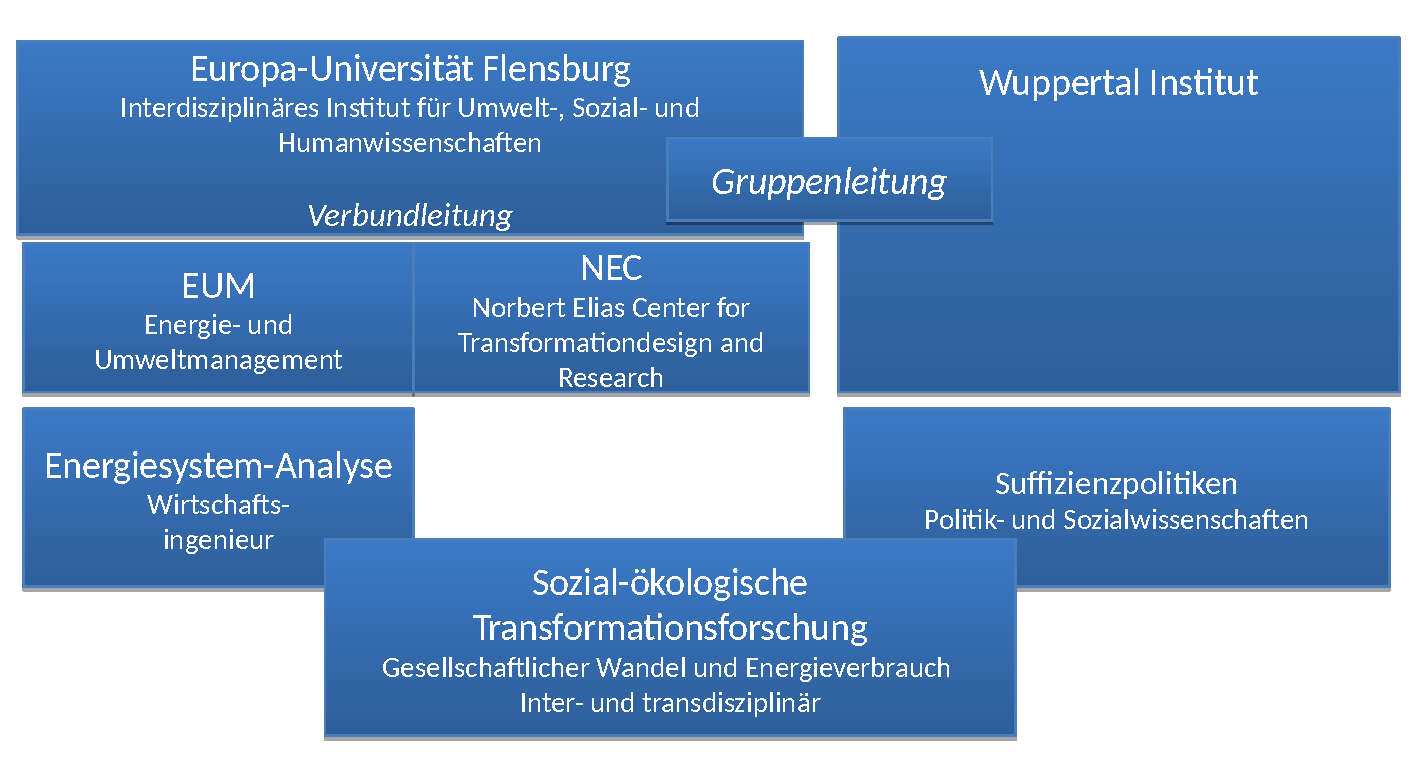
\includegraphics[width=0.8\textwidth]{figures/Konsortium5.pdf}
    \caption{Konsortium}
    \label{fig:konsortium}
\end{figure}

% Allgemein EUF EUM NEC Wuppertal
Die Nachwuchsgruppe ist am interdisziplinären Institut für Umwelt-, Sozial- und Humanwissenschaften der Europa-Universität Flensburg (EUF) und dem WI für Klima, Umwelt, Energie angesiedelt (WI).
% Leitung geteilt
Zur Verstärkung des interdisziplinären Charakters und der engeren Kooperation zwischen Universität und außeruniversitärer Forschungseinrichtung, wird die Forschungsgruppe gemeinsam von Frauke Wiese (EUF) und Benjamin Best (WI) geleitet.\\
Der Forschungs-Schwerpunkt Energiesystem-Analyse ist in der Abteilung Energie- und Umweltmanagement (EUM) der EUF verortet, während am WI wird der Forschungs-Schwerpunkt Suffizienz-Politiken bearbeitet wird. Das NEC (EUF) schlägt mit der sozial-ökologischen Transformationsforschung den inhaltlichen Bogen zwischen Wirtschaftsingenieurwesen und Politikwissenschaft. Abbildung \ref{fig:konsortium} stellt die Zusammenarbeit des Konsortiums dar.\\
Weitere Kooperationen außerhalb der Verbundpartner bestehen bereits im Suffizienz-Forschungsnetzwerk und dem inter- und transdisziplinären Netzwerk Vorsorgendes Wirtschaften. Der Bereich Energiesystemanalyse bringt die bereits bestehende Forschungskooperationen mit der Open Energy Modelling Initiative \cite{openmod} ein.\\
% Praxispartner
Desweiteren ist eine enge Zusammenarbeit mit kommunalen Praxispartnern bei der Szenarienerstellung und -bewertung geplant. Welche Praxispartner*innen im Nachwuchsforschungsvorhaben in welcher Weise eingebunden werden hängt von der empirischen und theoretischen Schwerpunktsetzung der Qualifikationsarbeiten ab.

\section{Betreuungskonzept}
%\textit{(inklusive der/des vorgesehenen Mentorin bzw. Mentors und Nachweis deren/dessen Expertise in Bezug auf inter- und transdisziplinäre Forschung}
Qualifikationsprozesse bergen zumeist ein Element der „Zwangsisolation“. Daher stellen Nachwuchsprojekte eine vorzügliche Möglichkeit zur Vernetzung und zum Austausch dar. Gleichwohl gilt es zwischen ruhigen Arbeitsphasen (bis hin zur Klausur) und gemeinsamen Treffen und Veranstaltungen auszubalancieren. Das Betreuungskonzept sieht vor, die Wachstumsringe der einzelnen Personen und deren Qualifizierungsarbeiten ebenso zu begleiten wie die gemeinsamen Prozesse zu unterstützen.
Die Gruppenleiterin Frauke Wiese betreut die Promotion in der Energiesystemanalyse; der Projektleiter des WIs Benjamin Best die Promotionen im Bereich Suffizienz-Politiken, während die fachliche Betreuung der beiden Promotionen im Bereich sozial-ökologische Transformationsforschung im Rahmen des Transformationskollegs des NECs erfolgt (Leitung: Prof. Dr. Harald Welzer, Koordination und Organisation: Dr. Michaela Christ und Dr. Bernd Sommer) und von jeweils einer der Gruppenleiter*innen interdisziplinär unterstützt wird. Bei der anspruchsvollen Betreuungsaufgabe im Spagat zwischen den Disziplinen unterstützen sich die beiden Nachwuchsgruppenleiter*innen gegenseitig und werden dabei zugleich von der Mentorin unterstützt. Vorgesehen ist Prof. Dr. Uta v. Winterfeld (WI und demnächst auch Universität Kassel), weil sie sowohl disziplinär und formal betreuen als auch inter- und transdisziplinär mitwirken kann (siehe CV im Anhang).\\
Zweimal im Jahr findet ein Reflexionstreffen der Gruppenleiter*innen und der Mentorin statt mit Fokus auf die Rolle als Leiter*in und den allgemeinen Fortschritt der Forschungsgruppe. Ebenso halbjährlich findet ein Treffen aller Mitarbeiter*innen der Nachwuchsforschungsgruppe einschließlich der Mentorin statt, in der jede*r den Fortschritt des Promotionsprojektes vorstellt. So werden nächste Schritte interdisziplinär geprüft und Probleme können frühzeitig erkannt und diskutiert werden.\\
Umwelt- und Transformationsforschung sind per se inter- und transdisziplinär angelegt. Gleichwohl hat sich gezeigt, dass wenig hilfreich ist, wenn alle Beteiligten von ihren Disziplinen absehen und sich naiv gutwillig in einem nicht näher bestimmten inter- und transdisziplinären Raum bewegen. Daher ist das Betreuungskonzept so angelegt, dass einerseits disziplinäre Vergewisserungen erfolgen und andererseits eine Kultur der interdisziplinären Öffnungen gepflegt wird. Hierzu gehört auch, unterstützt durch Weiterbildungsangebote, den disziplinären Blick auf gemeinsame Forschungsgegenstände wie beispielsweise private Haushalte zu werfen. Transdisziplinär wird auf der Betreuungsebene darauf geachtet, dass Praxispartner*innen in den Qualifizierungsarbeiten nicht zu Forschungsobjekten degradiert werden, die ihrerseits im Prozess keine Stimme haben. Vielmehr wird die Subjekt-Objekt-Dialektik kritisch reflektiert. Auch hierzu soll es Weiterbildungsmöglichkeiten geben, die sowohl durch vom Verbund eingeladene Expert*innen als auch durch die Teilnahme an Summer Schools o.Ä. erfolgen kann.\\ 
Die akademische Qualifizierung der Nachwuchswissenschaftler*innen wird sowohl durch Möglichkeiten der Zweitbetreuung von Bachelor- und Masterarbeiten unterstützt als auch dadurch verstärkt, dass von Anfang an eine Kultur des Publizierens gepflegt wird, die in kumulative Promotionen münden können.

\section{Institutionen, Zukunftsperspektiven und Ergebnisverwertung}
%\textit{Darstellung und Motivation der beteiligten Institutionen sowie Zukunftsperspektiven für die jeweiligen Mitglieder der Nachwuchsgruppe (nicht grundfinanzierte außeruniversitäre Forschungsinstitute haben zusätzlich darzustellen, inwieweit den betreffenden Mitgliedern zeitlich befristete Freiräume eingerichtet werden können, sich zeitweise voll auf ihre Qualifikation zu konzentrieren), erwartetes Ergebnis, Anwendungspotenzial und angestrebte Ergebnisverwertung. Der Verwertungsplan muss konkrete Maßnahmen der Öffentlichkeitsarbeit und des Wissenstransfers (auch von Zwischenergebnissen) beinhalten}
% EUF
An der EUF wurde mit der Einrichtung des Interdisziplinären Instituts für Umwelt-, Sozial- und Humanwissenschaften eine zentrale institutionelle Struktur für disziplin-übergreifende Fragestellungen geschaffen. Die Verankerung der sozial-ökologischen Forschung in Form einer eigenständigen Nachwuchsgruppe würde diese mit dem konkreten Forschungsthema Energiesuffizienz mit Leben füllen. Die Zusammenarbeit der wirtschaftsingenieur-lastigen Abteilung Energie- und Umweltmanagement sowie des sozialwissenschaftlich geprägten NEC gilt als große Bereicherung und fügt sich sowohl in die Forschungsarbeit des Interdisziplinären Instituts für Umwelt-, Sozial- und Humanwissenschaften, als auch in das Leitbild der EUF ausgezeichnet ein. Die Stärkung der inter- und transdisziplinären Forschung und insbesondere des Themenschwerpunktes Energiewende und Gesellschaft entspricht der Identität und der zukünftigen Entwicklung der Hochschule.\\
% WI
Das WI arbeitet interdisziplinär und problemlösungsorientiert im Themenbereich der angewandten Nachhaltigkeitsforschung. Seine Aufgabe ist die Wahrnehmung einer Mittlerfunktion zwischen Wissenschaft, Wirtschaft und Politik. Aus dem Spannungsfeld des Institutsauftrages – zwischen wissenschaftlichem Erkenntnisinteresse und geforderter Umsetzungsrelevanz der entwickelten Vorschläge – ergibt sich eine breite Forschungsagenda. Die Forschungsarbeiten bauen auf disziplinären wissenschaftlichen Erkenntnissen auf und verbinden diese bei der transdisziplinären Bearbeitung komplexer Fragestellungen zu praxisrelevanten und akteursbezogenen Lösungsbeiträgen. Das WI hat den Suffizienzbegriff 1993 in die deutsche Debatte eingebracht (Wolfgang Sachs) und forscht seit einigen Jahren intensiv im Bereich der Suffizienz- und Energiesuffizienzpolitiken. Es hat Kooperationsbeziehungen vor allem mit den Universtäten Wuppertal und Kassel; eine Intensivierung der Zusammenarbeit mit der EUF ist ebenso naheliegend wie erwünscht.\\
% Zukunftsperspektiven für die jeweiligen Mitglieder
Nach Ablauf des Projektes werden die Nachwuchswissenschaftler*innen mit ihrer inter- und transdisziplinären Erfahrung in einem gesellschaftlich hochaktuellen Thema bestens aufgestellt sein um ihre wissenschaftliche Karriere in diesem Bereich weiterzuführen. An der EUF werden durch eine perspektivische Verstetigung des Forschungsfeldes 'Gesellschaftliche Transformation und Energiewende' Optionen für eine interdisziplinäre akademische Laufbahn in diesem Bereich geschaffen; am WI können außeruniversitäre mit universitären Laufbahnen kombiniert werden. In der letzten Phase der Nachwuchsforschungsgruppe wird der Zukunftsplanung und Analyse der Optionen und Folge-Projekte der beteiligten Wissenschaftler*innen Raum gegeben.\\
% Welches Ergebnis erwarten wir und wie kann es von Forschung und Zivil-Gesellschaft genutzt werden?
Die erarbeiteten Methoden zur konsistenten, integrativen und zur qualitativen Seite hin offenen Szenarienerstellung kann von anderen, speziell interdisziplinär arbeitenden Forscher*innen angewendet und weiterentwickelt werden. Auch das Energiesystem-Modell, dessen Programmier-Code und Daten open source zur Verfügung gestellt wird, bildet eine Basis um auf den Erkenntnissen zu Energie-Suffizienz aufzubauen. 

\textit{MICHAELA BITTE EIN SATZ EINFÜGEN}\\
Die Zukunftserzählungen... 

Die Forschungsarbeiten am WI werden Erkenntnisse zu Blockaden für und Potenzialen von Energiesuffizienz-Politiken generieren und damit politische wie zivilgesellschaftliche Transformations- und Innovationsprozesse stärken.

%OPEN DATA und OPEN SOURCE
%Im Rahmen des Projektes erarbeitete Daten und Software, werden open source zur Verfügung gestellt. Der Open Science Ansatz, der der Nachwuchs-Forschungsgruppe zugrunde liegen wird, beinhaltet auch den offenen Zugang zu Publikationen etc. Die Erkenntnisse sollen außerdem politische Entscheidungsprozesse zu Klimaschutz und Energiewende unterstützen und Empfehlungen für Suffizienzpolitik beinhalten. Ein Schwerpunkt wird die Ergebnis-Kommunikation auch im populär-wissenschaftlichen Bereich, um auch eine außerwissenschaftliche Öffentlichkeit zu erreichen.

% Öffentlichkeitsarbeit und Wissenstransfer (konkrete Maßnahmen)
Der wissenschaftliche Wissenstransfer wird durch die Teilnahme an Konferenzen und Workshops sowie an Forschungsnetzwerken (Energiewende, Vorsorgendes Wirtschaften, Suffizienz, open energy modelling) sichergestellt. Im Rahmen des Projektes erarbeitete Daten und Software, werden open source zur Verfügung gestellt. Der Open Science Ansatz, der der Nachwuchs-Forschungsgruppe zugrunde liegen wird, beinhaltet auch den offenen Zugang zu Publikationen etc. Ein Lernziel der Nachwuchsforschung ist nicht nur die wissenschaftlichem Verschriftlichung, sondern auch die Kommunikation der Forschungsergebnisse an Nicht-Wissenschaftler*innen. Der Wissenstransfer soll in Form eines Blogs zum Thema Energie-Suffizienz im weiteren Sinne, einer Ringvorlesung sowie der Teilnahme der Wissenschaftler*innen an Formaten wie ``Science Slam'' geschehen. Die Workshops mit den Praxispartnern sind auch Teil der Öffentlichkeitsarbeit und dienen dem gegenseitigen Wissenstransfer von Zivilgesellschaft, Politik und Wissenschaft. Eine gemeinsame Exkursionsreihe 'Suffizienz-Beispiele in der Praxis' in Zusammenarbeit mit den Praxispartnern wird angestrebt.

\section{Zeitplanung und Kostenschätzung}
%\textit{Gesamtkosten bzw. -ausgaben, Grobkalkulation von Personal-, Sach- und Reisemitteln, gegebenenfalls Berücksichtigung von Eigenbeteiligung sowie Drittmitteln).}
%\textit{Basierend auf den geltenden tarifrechtlichen Regelungen und projektbezogen, können in der Regel maximal vier wissenschaftliche Personalstellen (teilbar) je Nachwuchsgruppe beantragt werden (davon maximal zwei Post-Doktorandinnen oder Post-Doktoranden). Bereits durch öffentliche Mittel grundfinanzierte Stellen können grundsätzlich nicht gefördert werden.
%In begrenztem Umfang können auch Assistenz- und Hilfskräfte sowie Sachmittel und Mittel zur Einbindung von Praxispartnern beantragt werden.}
Die zeitliche Einordnung und Abfolge der in Abschnitt \ref{sec:4} und Abbildung \ref{fig:forschungsprogramm} beschriebenen Arbeitspakete kann Abbildung \ref{fig:gantchart} entnommen werden. Die Kalkulation der Personal-, Reise-, Sach- und Weiterbildungsmittel sind Tabelle \ref{tab:kostenkalkulation} zu entnehmen. Tabelle \ref{tab:kostenkalkulation2} fasst die Kosten je Institution sowie die beantragte Zuwendung entsprechend der Förderquote zusammen.
\begin{figure}[ht!]
\begin{center}
\resizebox{0.95\textwidth}{!}{
    \begin{ganttchart}[hgrid,
    	vgrid={*{2}{draw=none},dotted},
    	x unit=.65cm,
    	y unit chart=1.75cm,
    	time slot format=isodate-yearmonth,
    	compress calendar,
    	bar/.append style={draw=none,fill=blue},
    	title label font=\Huge\bfseries,
    	group label font=\Huge\bfseries,
    	group/.append style={draw=none,fill=black!50!white},
    	milestone/.append style={draw=none,fill=orange},
    	bar height=.8,
    	group height=.35,
    	milestone height=.75,
    	milestone top shift=.1,
    	milestone label font=\color{orange}
    	]{2019-5}{2024-4}
    	%labels
    	\gantttitle{2019}{8}
    	\gantttitle{2020}{12}
    	\gantttitle{2021}{12}
    	\gantttitle{2022}{12}
    	\gantttitle{2023}{12}
    	\gantttitle{2024}{4} \\
    	\gantttitle{Jahr 1}{12}
    	\gantttitle{Jahr 2}{12}
    	\gantttitle{Jahr 3}{12}
    	\gantttitle{Jahr 4}{12}
    	\gantttitle{Jahr 5}{12}\\
    	%\gantttitle{2}{5}
    	%\gantttitle{3}{5}
    	%\gantttitle{4}{5}
    	%\gantttitle{1}{5}
    	%\gantttitle{2}{5}
    	%\gantttitle{3}{5}
    	%\gantttitle{4}{5} \\
    	%tasks
        \ganttgroup{AP 1}{2019-5}{2020-4}\\
         %   \ganttgroup{}{2020-10}{2021-9}\\
        \ganttgroup{AP 2}{2020-5}{2021-10}\\
        \ganttgroup{AP 3}{2021-1}{2022-4}\\
        \ganttgroup{AP 4}{2021-11}{2023-4}\\
        \ganttgroup{AP 5}{2022-11}{2023-10}\\
        \ganttgroup{AP 6}{2023-4}{2024-4}
    	% \ganttbar[bar/.append style={fill=red}]{AP1.1}{2018-12}{2018-04}\\
    	% \ganttmilestone[inline]{MS1}{2020-6}
    \end{ganttchart}
}
\end{center}
\caption{Gantt-Diagramm der Arbeitspakete}
\label{fig:gantchart}
\end{figure}
Für die gesamten fünf Jahre werden durchgängig vier Stellen beantragt von denen 1,75 Stellen am WI und 2,25 Stellen an der EUF verortet sind. Letztere setzen sich aus einer 0,75-Stelle für die Leitung und drei Doktoranden-Stellen zusammen (halbe Stellen). Am WI wird ebenso eine 0,75-Leitungsstelle (Zusammengesetzt aus 50\% Co-Leitung und 25\% Betreuungs- bzw. Mentor*innenarbeit, letztere für den gesamten Verbund, sowie zwei halbe Stellen als Doktorandenstellen eingeplant. Zusätzlich werden wissenschaftliche Hilfskräfte für 20 Stunden pro Woche und Forschungs-Schwerpunkt eingeplant. Es wird ein Overhead von 20\% für die EUF und von 90\% für die außeruniversitäre Forschungseinrichtung WI veranschlagt. Der Eigenanteil des WI beträgt 10\%.\\
In den Reisemitteln sind die Teilnahme an Konferenzen ab dem zweiten Jahr sowie an vier Workshops pro Person und Jahr enthalten. Außerdem wurde mit halbjährlichen Treffen in abwechselnd Wuppertal und Flensburg mit allen Personen und zusätzlichen drei bilateralen Treffen pro Jahr kalkuliert. In den Sachmitteln sind neben Literatur und Computer für die Modellierung ab dem zweiten Jahr Gelder für Open Access Veröffentlichungen enthalten. In die Kategorie Weiterbildung fallen Kursgebühren für Qualifizierungsworkshops und Summer Schools.

\begin{table}[h]
\begin{center}
  \caption{Abschätzung der Gesamtkosten je Kostenkategorie für Energie- und Umweltmanagement (EUM) und Norbert Elias Center (NEC) (beide interdisziplinäres Institut der Europa-Universität Flensburg (EUF)) und Wuppertal Institut}
\small  
\begin{tabular}[h]{|l | r | r | r | r|}
\hline
&&&&\\
& EUF EUM & EUF NEC & Wuppertal Institut & \textbf{Summe in Euro}\\
\hline
\hline
&&&&\\
 Personalmittel & 622.540 & 495.080 & 1.474.710 & 2.592.330\\
 \hline
 &&&&\\
 Reisemittel & 54.000 & 54.000 & 50.000 & 158.000\\
 \hline
 &&&&\\
 Sachmittel & 28.200 & 28.200 & 30.000 & 86.400\\
 \hline
 &&&&\\
 Weiterbildung & 15.600 & 15.600 & 15.000 & 46.200\\
 \hline
 \hline
 &&&&\\
 \textbf{Summe}& \textbf{720.340} & \textbf{592.880} & \textbf{1.569.710} & \underline{\textbf{2.882.930}}\\
 \hline
 \end{tabular}
 \label{tab:kostenkalkulation}
\end{center}
\end{table}

\begin{table}[h]
\small
\begin{center}
  \caption{Abschätzung von Gesamtkosten und beantragter Förderung je Institution}
\begin{tabular}[h]{|l | r | r | r|}
\hline
&&&\\
Institution & Kosten [Euro] & Förderquote [\%] & \textbf{beantragte Zuwendung}\\
\hline
\hline
 &&&\\
 EUF & 1.313.220 & 100 & 1.313.220\\
 \hline
 &&&\\
 Wuppertal Institut & 1.569.710 & 90 & 1.412.739
\\
 \hline
 \hline
 &&&\\
 \textbf{Gesamt} & & &\underline{\textbf{2.725.959}}\\
 \hline
 \end{tabular}
 \label{tab:kostenkalkulation2}
\end{center}
\end{table}

\clearpage

%\sectionp*{Literatur} \label{sec:lit}
%\bibliographystyle{plainnat}%elsarticle-num}
\bibliographystyle{elsarticle-num}
%\bibliographystyle{apalike}
\bibliography{literature.bib}

\clearpage
\appendix

\section{Anhang}

\textit{Literaturlisten, Lebensläufe und gegebenenfalls Interessensbekundungen von Praxispartnern sind im Anhang beizufügen.}

\section{Projekte}
Für die Übersicht sind die Projekte hier nochmal aufgeführt


\section{Lebensläufe}
%Formatierung / Kürzung überlasse ich gern Dir, Frauke

Dr. des. Benjamin Best 

Benjamin Best ist seit 2011 wissenschaftlicher Mitarbeiter am Wuppertal Institut in der Abteilung Zukünftige Energie- und Mobilitätsstrukturen. Er arbeitet im interdispziplinären Forschungsprojekt DoNaPart, welches im Rahmen von BMBF-SÖF / Zukunftsstadt gefördert wird und Erkenntnisse gewinnen möchte, wie durch gemeinschaftliches Handeln nachhaltige und lebenswerte Städte geschaffen werden können. Best ist zudem seit 2014 am "Virtuellen Institut - Energiewende NRW" beteiligt, in dem nicht-technische Energieforschungsprojekte in NRW gebündelt werden. 
Best hat Soziologie, Geschichte (B.A.) und Sustainability Economics and Management (M.A.) in Oldenburg studiert. Er hat Ende April 2018 seine Doktorarbeit im Fach Politikwissenschaft an der Bergischen Univesität Wuppertal erfolgreich verteidigt. Best war 2014 Mitglied im Organisationskreis der „International Degrowth Conference“ in Leipzig und ist Juror des Karl W. Kapp-Forschungspreises für Ökologische Ökonomie. 

%Für die Entwicklung von Alternativen hierzu ist Benjamin Best als Ko-Leiter durch seine Arbeiten in den Projekten Innovation City (Bottrop) und im sozial-ökologischen Forschungsverbund DoNaPart (\url{https://projekt-donapart.de/}) gut ausgestattet. 

% (z.B. im Rahmen der Entwicklung des Klimaschutzplans NRW (Suffizienz wurde als Klimaschutzsstrategie in der Arbeitsgruppe „Private Haushalte“ diskutiert, welche u.a. von Benjamin Best begleitet wurde. \url{https://wupperinst.org/p/wi/p/s/pd/376/} und \url{https://wupperinst.org/p/wi/p/s/pd/396/}, interdisziplinärer Modellierung z.B. im Rahmen des Projektes COMBI \url{https://combi-project.eu/} sowie in der methodischen Entwicklung zur Integration sozialwissenschaftlicher Empirie in die Modellierung \cite{Bierwirth2016}.\\

%Benjamin Best bringt hierfür als interdisziplinärer ausgebildeter Soziologe mit technischer und sozialwissenschaftlicher Expertise hervorragende Voraussetzungen für die Ko-Leitung mit. Die sozialwissenschaftliche Seite wird durch ein volkswirtschaftliches und ein politikwissenschaftliches Promotionsvorhaben (Politische Ökonomie, Internationale Politik, Politische Ökologie) gestärkt. Die Wirtschaftsingenieurin Frauke Wiese bringt ihre langjährige Erfahrung in der Energiesystem-Modellierung und den technisch-ökonomischen Blickwinkel auf die Herausforderungen der Energiewende ein. 

% weitere Veröff Projekt Energiesuffizienz
%https://energiesuffizienz.files.wordpress.com/2014/10/thema-kg-analyse.pdf
%https://energiesuffizienz.files.wordpress.com/2014/12/arbeitspapier-breitenbefragung-160513.pdf
%Zu Politiken auch:
%https://energiesuffizienz.files.wordpress.com/2014/06/energiesuffizienzpolitik_20161212.pdf

\end{document}